%pdflatex -shell-escape vol.tex 
%pdflatex -shell-escape *.tex
\documentclass{standalone}
\usepackage{amsmath,amsfonts,amssymb}
%
\usepackage{graphicx}
\graphicspath{ {images/} }
%
\usepackage{xcolor}
\pagestyle{empty}
\pagecolor{white}
%
\everymath{\displaystyle}
%
\usepackage{CJKutf8}   %CJKspace
\AtBeginDvi{\input{zhwinfonts}}
%%%
\newcommand{\zh}[1]{\begin{CJK*}{UTF8}{zhsong}#1\end{CJK*}}
\newcommand{\YBao}{\color{red}\zh{源宝爱数学}}
\newcommand{\BT}[1]{\color{red}\zh{#1}\color{black}}
\newcommand{\fTxT}[1]{\text{\zh{#1}}}
%

\immediate\write18{pdflatex vol.tex}
\immediate\write18{convert -density 150 -adaptive-resize 480x480 vol.pdf vol.jpg}
%
\newcommand{\XB}[1]{\text{\zh{#1}}}
% 
\usepackage{pgfplots}
\pgfplotsset{width=100pt,compat=1.9}
% 
\begin{document}\begin{minipage}[b][14cm][t]{\textwidth}
%
\begin{minipage}{\linewidth}
\centering
\begin{tabular}{|c|l|l|}
\multicolumn{3}{c}{\Large\BT{面积与体积:(Area \& Volumn)}} \\[5pt] \hline
\BT{几何体} & \multicolumn{1}{c}{\BT{表面积}} & \multicolumn{1}{c}{\BT{体积}} \\ \hline
\zh{棱柱} & $S_\XB{侧}+2S_\XB{底}$
  & $S_\XB{底} \times h_\XB{高}$ \\ \hline
\zh{棱锥} & $S_\XB{侧}+S_\XB{底}$
  & $\frac{1}{3} \times S_\XB{底} \times h_\XB{高}$ \\ \hline
\zh{棱台} & $S_\XB{侧}+S_\XB{上底}+S_\XB{下底}$
  & $\frac{1}{3}(S_\XB{上底}+S_\XB{下底}+\sqrt{S_\XB{上底}S_\XB{下底}})h_\XB{高}$ \\ \hline
\zh{圆柱} & $2\pi r^2 + 2\pi rh$ & $\pi r^2 h$ \\ \hline
\zh{圆锥} & $\pi r^2 + \pi rl$ & $\frac{1}{3}\pi r^2 h$ \\ \hline
\zh{圆台} & $\pi (r_\XB{上底}^2 + r_\XB{下底}^2 + r_\XB{上底}l + r_\XB{下底}l)$ & $\frac{1}{3}\pi (r_\XB{上底}^2 + r_\XB{下底}^2 + r_\XB{上底} r_\XB{下底})h_\XB{高}$ \\ \hline
\zh{球}   & $4\pi R^2$ & $\frac{4}{3}\pi R^3$ \\ \hline
\multicolumn{3}{l}{\zh{斜二测所画图形面积}=\zh{原图形面积}$\times\frac{\sqrt 2}{4}$} \\ \hline
\end{tabular}\end{minipage} \\[7pt]
%%%
\begin{minipage}{\linewidth}
\centering
\begin{tabular}{|l|l|}
\multicolumn{2}{c}{\Large\BT{判定、性质定理}} \\ \hline
\multicolumn{1}{c}{\BT{线面平行}} &
\multicolumn{1}{c}{\BT{线面垂直(两垂一相交)}} \\ \hline
  $\left.\begin{aligned}
    a \not\subset \alpha\\
    b \subset \alpha\\
    a // b
  \end{aligned}\right\} \Longrightarrow a \| \alpha$
& $\left.\begin{aligned}
    a,b \subset \alpha\\
    a \cap b = A\\
    c \perp a, c \perp b\\
  \end{aligned}\right\} \Longrightarrow c \perp \alpha$ \\ \hline
\multicolumn{1}{c}{\BT{面面平行}} & 
\multicolumn{1}{c}{\BT{面面垂直}} \\ \hline
  $\left.\begin{aligned}
    l_1,l_2 \subset \alpha, l_1 \cap l_2 = A\\
    l_3,l_4 \subset \beta,  l_3 \cap l_4 = B\\
    l_1 \| l_3, l_2 \| l_4\\
   \end{aligned}\right\} \Longrightarrow \alpha \| \beta$
& $\left.\begin{aligned}
    c \subset \alpha\\
    c \perp \beta
\end{aligned}\right\} \Longrightarrow \alpha \perp \beta$ \\ \hline
\end{tabular}\end{minipage} \\[7pt] 
%%%
\begin{minipage}{\linewidth}
\centering
\begin{tabular}{ll}
\multicolumn{2}{c}{\BT{爱你(Love You)}}\\ \hline
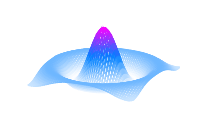
\begin{tikzpicture}
\begin{axis}[
    %title=Exmple using the mesh parameter,
    hide axis,
    colormap/cool,
]
\addplot3[
    mesh,
    samples=50,
    domain=-8:8,
]
{sin(deg(sqrt(x^2+y^2)))/sqrt(x^2+y^2)};
%\addlegendentry{$\frac{sin(r)}{r}$}
\end{axis}
\end{tikzpicture}
&
  \includegraphics{ybao30.jpg}
\end{tabular}\end{minipage}
%
\end{minipage}\end{document}
